\subsection{A triangulação de Delaunay e o diagrama de Voronoi}
\label{cap_triangulacao_delaunay}

Nesta seção, aborda-se a triangulação de Delaunay e o diagrama de Voronoi. Também são apresentados algoritmos de construção, manutenção e refinamento dessa triangulação.

\subsubsection{Considerações iniciais}

Uma malha pode ser classificada de acordo com a disposição relativa dos diferentes elementos existentes. Uma malha {\it estruturada} é caracterizada pela sua conectividade {\it regular}. Isso significa que, a posição dos nós pode ser mapeada de modo a definir quais nós serão vizinhos por meio de cálculo. Isso pode restringir as escolhas dos elementos para quadriláteros em 2D ou hexaedros em 3D. Se os nós não podem ser arranjados de tal forma, a malha é dita {\it não estruturada} ou {\it irregular}. Em uma malha irregular, deve-se armazenar a conexão entre os nós que formam a malha. Os elementos podem ser, em sua forma básica, triângulos ou tetraedros em 2D e 3D, respectivamente, bem como hexaedros, ou qualquer outra forma, em malhas mais complexas. \cite[p.~20]{Thompson1999}.

Na busca de se atingir uma determinada qualidade na aproximação, com desempenho computacional aceitável, ao longo das últimas décadas, pesquisas têm sido realizadas em técnicas de geração e refinamento de malhas, como por exemplo em \citeonline{Preparata1985, Thompson1999, Teng2000, Chen2004, George2008}. Ainda em problemas com domínios com geometria complexa, a geração da malha pode ser uma tarefa dispendiosa. Uma forma de se obter uma malha de qualidade a baixo custo computacional é a utilização da triangulação Delaunay. 

A triangulação de \citeonline{Delaunay1939} é um tipo de malha irregular. Com uma triangulação de Delaunay, maximiza-se o menor ângulo da triangulação. Obtém-se triângulos com ângulos não próximos a $0^{\circ}$ e a $180^{\circ}$. Em esquemas numéricos, triângulos com ângulos próximos a $0^{\circ}$ e $180^{\circ}$ são considerados de má qualidade, levando a resultados imprecisos. 

A triangulação de Delaunay possui a característica de unicidade, de forma que, dado um conjunto de vértices, a triangulação é sempre única, exceto em casos degenerados, nos quais quatro ou mais vértices são cocirculares, existindo duas possibilidades de triangulação (local). Cada uma das duas possibilidades de triangulação que divide o quadrilátero em dois triângulos satisfaz a ``condição Delaunay'', isto é, em que o circuncírculo (único círculo que passa pelos vértices do triângulo) é vazio. Essa noção pode ser estendida a três dimensões.

Um diagrama de \citeonline{Voronoi1908} é uma decomposição (em partições) de um espaço em torno de um vértice. Cada polígono consiste em uma região de espaço que fica mais próxima de cada vértice do que qualquer outro vértice gerador do diagrama de Voronoi, que é formado pelos polígonos de Voronoi. Diversos algoritmos para a geração do diagrama de Voronoi foram desenvolvidos. São exemplos desses algoritmos, \citeonline{Shamos1975}, que desenvolveram um algoritmo O($n\cdot \mbox{lg}(n)$) por divisão-e-conquista e \citeonline{Green1978}, que produziram um algoritmo O($n^2$) por inserção incremental, em que $n$ é a quantidade de vértices da triangulação.

Uma partição do diagrama de Voronoi e a triângulação de Delaunay correspondente pode ser observada na figura (\ref{fig_malha_voronoi}).

\begin{figure}[!ht]
  \centering
  \includegraphics[width=150pt]{imagens_discretizacao/malha_voronoi.png}
  \caption{\footnotesize{Em azul, arestas de uma partição do diagrama de Voronoi e, em vermelho, os triângulos de Delaunay correspondentes.
}}
  \label{fig_malha_voronoi}
\end{figure}

\subsubsection{Manutenção da triangulação de Delaunay - Algoritmo de Lawson}
\label{cap_algoritmo_lawson}
Para construção da triangulação Delaunay, pode-se utilizar o algoritmo de \citeonline{Lawson1977}, um algoritmo de complexidade $O(n^2)$. Esse algoritmo é utilizado para gerar ou para manter uma triangulação de Delaunay. Sua escolha deve-se à sua facilidade de implementação.

A partir de uma triangulação inicial, verifica-se se todas as arestas que compõem a triangulação atendem aos critérios da triangulação de Delaunay. Caso essas arestas não atendam aos critérios da triangulação de Delaunay, realiza-se o {\it flip}. 

O {\it flip} é um procedimento, definido por \citeonline{Lawson1977}, em que ocorre a inversão da aresta invadida, conforme demonstrado na figura (\ref{fig_flip}). Com o {\it flip}, uma nova aresta é criada e, em seguida, verifica-se, recursivamente, essa aresta e os dois triângulos que a compartilham. O algoritmo termina quando todas as arestas atendem aos critérios da triangulação de Delaunay, ou seja, são localmente de Delaunay.  

\begin{figure}[!ht]
  \centering
  \includegraphics[width=350pt]{imagens_delaunay/novo_flip.png}
  \caption{\footnotesize{Aplicação do algoritmo de Lawson: (a) Uma aresta invadida, mostrada em vermelho, que não é de Delaunay, é verificada. (b) O algoritmo do {\it flip} é aplicado para inverter a aresta invadida, tornando-a localmente de Delaunay. (c) Verifica-se se essa aresta e os dois triangulos que a compartilham são localmente de Delaunay. Como a aresta não é invadida, essa é mostrada em azul.
}}
  \label{fig_flip}
\end{figure}

No algoritmo (\ref{algoritmo_lawson}) tem-se um pseudocódigo referente ao algoritmo de \citeonline{Lawson1977}.

\begin{algorithm}[!ht]
\caption{Algoritmo de Lawson.} 
\label{algoritmo_lawson}
\Entrada{Triangulação $T$.}
\Saida{Triangulação de Delaunay $T$.}
  \Inicio{
    \Para {(cada aresta $\overline{ab} \in T$)} {
    \CommentSty{// Efetua teste do circuncírculo.} \\
      \Se {($\overline{ab}$ não é localmente de Delaunay)} {
	  Sejam $\Delta abc$ e $\Delta abd$ os triângulos que compartilham $\overline{ab}$; \\
	  Trocar $\overline{ab}$ por $\overline{cd}$; \CommentSty{// Realiza o {\it flip} da aresta.}\\
      }
    }
    \Retorna {$T$;}
  }
\end{algorithm} 

\subsubsection{Construção da triangulação de Delaunay - Algoritmo de Green-Sibson}
\label{cap_algoritmo_green_sibson}

O algoritmo de Green-Sibson foi proposto por \citeonline{Green1978} para gerar o diagrama de Voronoi, porém, pode ser facilmente adaptado para gerar a triangulação de Delaunay. A partir de uma triangulação de Delaunay inicial realiza-se a inserção incremental de vértices.  Os pontos inseridos na triangulação de Delaunay são chamados de pontos de {\it  Steiner}. A complexidade desse algoritmo é $O(n^2)$.

Nesse algoritmo, ocorre a inserção de um vértice por vez e, a cada inserção, verifica-se se o novo vértice encontra-se sobre uma aresta ou dentro de um triângulo. Caso o novo vértice $e$ se localize dentro do triângulo $\Delta abc$, liga-se $e$ aos três vértices do triângulo que o contém, criando-se três novos triângulos, $\Delta abe$, $\Delta ace$ e $\Delta bce$. Caso o novo vértice $f$ se localize sobre uma aresta $\overline{de}$, deve-se dividir $\overline{de}$ em duas novas arestas. Considere $\Delta bde$ e $\Delta cde$ os triângulos que compartilham $\overline{de}$. Divide-se a aresta $\overline{de}$ em duas novas arestas, $\overline{ef}$ e $\overline{df}$. Em seguinda, liga-se $f$ aos vértices $b$ e $c$, opostos à aresta $\overline{de}$, pertencentes aos triângulos que compartilham $\overline{de}$, criando-se quatro novos triângulos, $\Delta bef$, $\Delta bdf$, $\Delta cef$ e $\Delta cdf$. Em ambos os casos realiza-se o teste do circuncírculo após a geração das novas arestas, utilizando o algoritmo de \citeonline{Lawson1977} para manutenção da malha. Se existirem arestas invadidas, realiza-se o {\it flip}. O algoritmo termina quando não existirem arestas invadidas. Na figura (\ref{fig_green_sibson}), pode-se observar um exemplo de execução do algoritmo de \citeonline{Green1978} 

No algoritmo (\ref{algoritmo_green_sibson}) tem-se um pseudocódigo referente ao algoritmo de \citeonline{Green1978}.

\begin{figure}[!ht]
  \centering
  \includegraphics[width=350pt]{imagens_delaunay/green_sibson.png}
  \caption{\footnotesize{Aplicação do algoritmo de Green Sibson: (a) Tem-se a malha inicial com a inserção de um novo vértice que localiza-se dentro de um triângulo. (b) Divide-se o triângulo gerando três novos triângulos, formados pelas arestas em azul. (c) Realiza-se o teste dos circuncírculos e encontra-se uma aresta invadida, mostrada em vermelho. (d) Efetua-se o {\it flip} na aresta invadida. (e) Realiza-se o teste dos circuncírculos. (f) Ocorre a inserção de um novo vértice localizado sobre uma aresta. (g) Ocorre a divisão da aresta que contém o novo vértice, gerando quatro novos triângulos, compostos pelas novas arestas em azul. (h) Realiza-se o teste dos circuncírculos e verifica que não existe aresta invadida.
}}
  \label{fig_green_sibson}
\end{figure}

\begin{algorithm}[!ht]
\caption{Algoritmo de Green-Sibson.} 
\label{algoritmo_green_sibson}
\Entrada{Triangulação de Delaunay $TD$ e lista $L_V$ de vértices a serem inseridos em $TD$.}
\Saida{$TD$ com os vértices pertencentes à $L_V$.}
  \Inicio{
    \Para {(todo vértice $v \in L_V$)} {
	Inserir $v$ em $TD$; \\
	\eSe {($v$ localiza-se sobre aresta $\overline{ab} \in TD$)} {
	    Sejam $\Delta abc$ e $\Delta abd$ os triângulos que compartilham $\overline{ab}$; \\
	    Criar as arestas $\overline{av}$, $\overline{bv}$, $\overline{cv}$, $\overline{dv}$ e inserir em $TD$; \\
	}
	{
	    Seja $\Delta abc$ o triângulo que contém $v$; \\
	    Criar as arestas $\overline{av}$, $\overline{bv}$, $\overline{cv}$ e inserir em $TD$; \\
	}
    }
    \Para {(cada aresta $\overline{ab}$ criada)} {
	AlgoritmoLawson($\overline{ab}$);\\
    }
    \Retorna {$TD$;}
  }
\end{algorithm} 

\subsubsection {Refinamento de Delaunay} 
\label{cap_algoritmos_refinamento}
Nesta seção, são apresentados dois algoritmos no estado da arte para o refinamento de Delaunay: algoritmo de \citeonline{Ruppert1995} e \emph{off-centers} \cite{Ungor2004, Ungor2009, Oliveira2012a}.


\textbf {Algoritmo de Ruppert}
\label{cap_algoritmo_ruppert}

O algoritmo de \citeonline{Ruppert1995} garante que todos os triângulos pertencentes à triangulação terão ângulos entre $\alpha$ e $\pi-2\alpha$, de forma que $\alpha$ pode ser um ângulo máximo de aproximadamente 20,7 graus. Ao se inserir um vértice na triangulação, duas operações são possíveis: dividir um segmento e dividir um triângulo. Ao se dividir um segmento, um vértice é inserido em seu ponto médio. Ao se dividir um triângulo, um vértice é inserido em seu circuncentro. Com isso, uma nova triangulação é realizada \cite{Oliveira2012a}. 

Um algoritmo para a geração da triangulação de Delaunay pode utilizar uma medida de qualidade. Uma possível medida de qualidade chama-se \emph{Circunradius-to-shortest Edge Radio} (CER), que é definida pela razão do raio do circuncírculo \emph{r} (\emph{circunraio}) do triangulo, pela menor aresta \emph{l} do triângulo. É especificado um limite superior $\rho=r/l$ para o CER de todos os triângulos da malha. A razão $\rho$ de um triângulo está relacionada com seu menor ângulo ${\alpha}$ pela fórmula ${\rho = 1/[2\cdot sen(\alpha)]}$. Quanto menor for a razão $\rho$, maior será o ângulo $\alpha$ do triângulo. Esse limite superior $\rho$ garantirá que não há triângulo na malha com ângulo menor que ${\arcsin(1/2\rho)}$ \cite{Pebay2003}. 

Esse algoritmo pode receber como parâmetro de entrada um grafo planar de linhas não curvas (\emph {Planar Straight Line Graph} - PSLG). Um PSLG é um conjunto de vértices e seus segmentos. Segmentos são arestas que não podem ser removidos. Claramente, os segmentos não se interceptam. Um segmento é considerado invadido quando um vértice incide dentro de seu círculo diametral. Um pseudocódigo referente ao algoritmo de \citeonline{Ruppert1995} é apresentado no algoritmo (\ref{algoritmo_ruppert}).

\begin{algorithm}[!ht]
\caption{Refinamento de Ruppert.} 
\label{algoritmo_ruppert}
\Entrada{PSLG $G$.}
\Saida{Triangulação de Delaunay de $G$ com todos os $\measuredangle \geq \alpha$.}
\Inicio{
    Adicionar um delimitador quadrado $D$ à $G$: \\
    \Inicio{
      Calcular os extremos de $G$: $x_{min}$, $y_{min}$, $x_{max}$, $y_{max}$; \\
      Seja $span(G) = \max(x_{max} - x_{min}, y_{max} - y_{min})$; \\
      Seja $D$ o quadrado de lado $3 \times span(G)$, centralizado em $G$;\\
      Adicionar os quatro segmentos de contorno de $D$ à $G$; \\
    }
    Seja a lista de segmentos $L_{S} =$ arestas de $G$; \\
    Seja a lista de vértices $L_{V} =$ vértices de $G$; \\
    Construir a triangulação de Delaunay inicial $TD(L_{V})$;\\
    \Repita{ (at\'e que nenhum segmento esteja invadido e nenhum $\measuredangle < \alpha$) } 
    {
        \CommentSty{// Divide todos os segmentos invadidos em seu\\ // ponto m\'edio.}  \\  
	\Enqto{ (existe algum segmento $s \in L_{S}$ invadido) }
	{
	    $DividirSegmento(s)$; 
	}
	\CommentSty{ // Verifica tri\^angulos com $\measuredangle  < \alpha$.}  \\  
	\Enqto{ (existe algum tri\^angulo $\delta \in TD(L_{V})$ com $\measuredangle  < \alpha$;) }
	{
	    Seja $c$ o circuncentro de $\delta$; \\   	    
	    \eSe { ($c$ invade algum segmento $s \in L_{S}$) } 
	    {		
	        \CommentSty{// Divide todos os segmentos invadidos\\ // em seu ponto m\'edio.}  \\  
		$DividirSegmento(s)$; \\
	    }	    
	    {
	        \CommentSty{// Divide tri\^angulos com $\measuredangle < \alpha$, em seu\\ // circuncentro, adicionando $c$ \`a $L_{V}$.}  \\  
		$DividirTriangulo(\delta)$; \\
	    }   
	}
    }
    \Retorna {Triangulação de Delaunay corrente $TD(L_{V})$;}
}
\end{algorithm}  

Nas situações em que o PSLG possui ângulos menores que $90^{\circ}$, o algoritmo tende a formar triângulos com ângulos muito agudos. \citeonline{Shewchuk1997} provou que o algoritmo irá parar para qualquer entrada com ângulos de, no mínimo, $60^{\circ}$.

\textbf {\emph{Off-centers}}
\label{cap_off_centers}

\citeonline{Ungor2004,Ungor2009} propôs um refinamento de Delaunay similar ao algoritmo de \citeonline{Ruppert1995}. Em seu trabalho, introduz-se um novo tipo de pontos de {\it Steiner}, chamados {\it off-centers}, como uma alternativa aos circuncentros, apresentando um novo algoritmo de refinamento de Delaunay. Caso um triângulo seja considerado de má qualidade, pela medida CER, o algoritmo tenta inserir o \emph{off-center}. Caso o \emph{off-center} invada algum segmento, então, o novo vértice é inserido no ponto médio desse segmento em vez do \emph{off-center}. Um pseudocódigo referente a esse algoritmo pode ser observado no algoritmo (\ref{algoritmo_ungor}).

\begin{algorithm}[!ht]
\caption{Refinamento de \"Ungor.} 
\label{algoritmo_ungor}
\Entrada{PSLG $G$.}
\Saida{Triangulação de Delaunay de $G$ com todos os $\measuredangle \geq \alpha$.}
\Inicio{
    Seja $TD$ a triangulação de Delaunay dos vértices de $G$; \\
    Calcular: \\
    \ \ $B = $candidados à {\it off-centers} que invadem algum segmento;\\
    \ \ $C = $candidados à {\it off-centers} que não invadem segmentos;\\
    \ \ $D = $candidados à ponto médio;\\
    \Enqto{ ($C \cup D) \neq$ vazio }
    {
	Escolher um ponto $c_{o} \in (C \cup D)$ e inserir $c_{o}$ na triangulação $TD$; \\ 
	\Se { ($c_{o}$ é ponto médio de um segmento $s$)}
	{
	    $DividirSegmento(s)$;\\
	}
	Atualizar $TD$ e recalcular $B$, $C$ e $D$;
    }    
    \Retorna {Triangulação de Delaunay corrente $TD$;}    
}
\end{algorithm}  

Para calcular o {\it off-center}, considera-se um triângulo $\delta$, de má qualidade, formado pelos vértices $p$, $q$ e $r$. A menor aresta de $\delta$ é $pq$ e o seu circuncentro é $c$. O {\it off-center} $c_{o}$ de $\delta$ é o seu circuncentro se o CER do triângulo formado pelos vértices  $p$, $q$ e $c$ for menor ou igual a um dado limite $\rho_{\alpha}$, em que $\rho_{\alpha}$ é a medida CER de um ângulo $\alpha$, conforme mostrado na figura (\ref{fig_off_center}.a). Caso contrário, o {\it off-center} $c_{o}$ será o ponto na bissetora da aresta, dentro do circuncírculo, que faz com que o CER do triângulo $\Delta pqc_{o}$ seja exatamente igual a $\rho_{\alpha}$. A bissetora da aresta é a linha que passa pelo ponto médio de uma aresta de um triângulo e pelo seu circuncentro. 

O círculo que passa pelos vértices da menor aresta $pq$, centrado no {\it off-center}, é chamando {\it off-circle}. Caso o triângulo $\delta$ tivesse duas arestas menores iguais, escolheria-se uma delas, arbitrariamente. 

\begin{figure}[!ht]
  \centering
  \includegraphics[width=300pt]{imagens_delaunay/off-center_A_B_rotulado.png}
  \caption{\footnotesize{ O {\it off-center} e o circuncentro do triângulo $\delta$, formado pelos vértices $p$, $q$ e $r$, são, respectivamente, $c_{0}$ e $c_{1}$. O circuncentro do triângulo formado pelos vértices $p$, $q$ e $c_{0}$ é $c_2$. Se $|c_{0} c_{2}| \leq \rho_{\alpha}|pq|$ então $c_{0} = c_{1}$, que é demonstrado em (a). Caso contrário, $c_{0} \neq c_{1}$. Nesse caso, calcula-se $c_{2}$ de forma que $|c_{0} c_{2}| = \rho_{\alpha}|pq|$, que é demonstrado em (b). O {\it off-circle} do triângulo $\delta$ é o circuncírculo em (a) e é mostrado em linhas tracejadas em (b). Figura adaptada de \citeonline{Ungor2004, Ungor2009}.
}}
  \label{fig_off_center}
\end{figure}

\citeonline{Ungor2004,Ungor2009} mostrou que seu algoritmo possui as mesmas garantias do algoritmo de Ruppert. Seus experimentos mostraram que seu algoritmo insere aproximadamente 40\% menos vértices que outros algoritmos de inserção no circuncentro e malhas 30\% menores em relação ao número de elementos.

\subsubsection{Resumo}

Nesta seção, apresentou-se a triangulação de Delaunay, um tipo de malha irregular que possui a propriedade de maximizar o menor ângulo da triangulação e o seu dual, o diagrama de Voronoi. 

Nas subseções (\ref{cap_algoritmo_lawson}), (\ref{cap_algoritmo_green_sibson}) e (\ref{cap_algoritmos_refinamento}) foram explanados um algoritmo para manutenção da triangulação de Delaunay, o algoritmo de \citeonline{Lawson1977}, um algoritmo para construção da triangulação de Delaunay, o algoritmo de \citeonline{Green1978}, e dois algoritmos para refinamento de Delaunay: o algoritmo de \citeonline{Ruppert1995} e \citeonline{Ungor2004,Ungor2009}.